\chapter{Rigidity of Minimally Rigid Circle Packings} % need to change title as it isn't quite right
\label{ch: 4}

\begin{flushleft}
If we were to relate this thesis to a video game, the previous chapters would be like the levels where we, the player, would need to get through in order to gain skills or powers. These levels would contain small, trivial enemies that we'd easily defeat and gain a set of valuable tools in order to progress the game.    
\end{flushleft}

\begin{flushleft}
This chapter then, would be the showdown between the main character and the final boss of the game! We'll need to call upon all of the experience gained, use every ounce of the strength developed and employ each weapon attained over the course of this journey in order to win this fight.
\end{flushleft}

\section{The Goal}

\begin{flushleft}
As it's been stated a few times leading up to this point, the project focuses on figuring out whether every minimally rigid graph has a circle packing that is infinitesimally rigid itself. It is a question for which we (currently) have no answer to, and it is an interesting one in nature because although we know that a packing such that the contact graph is isomorphic to the original graph exists by Theorem \ref{thm: circle packing theorem}, the contact graph isn't necessarily infinitesimally rigid, see Figure \ref{fig4: iso but not rig}. Our task in this chapter is to understand whether this is true or not. 
\end{flushleft}

\begin{flushleft} % argue this better
If we were to be pedantic, we would need to talk about the framework itself with respect to rigidity, and the graph which gives rise to this framework when talking about isomorphism. To avoid the confusion (and tediousness) this will cause, we shall use the words `graph' and `framework' interchangeably from now on. 
%As this chapter focuses on non-isomorphic infinitesimally rigid frameworks, we can talk about the framework itself with respect to rigidity, or the graph which gives rise to this framework when talking about isomorphism. At this stage, it does not matter which one we refer to, and therefore, we shall use the words `graph' and `framework' interchangeably. 
\end{flushleft}

\begin{figure}[htbp]
    \centering
    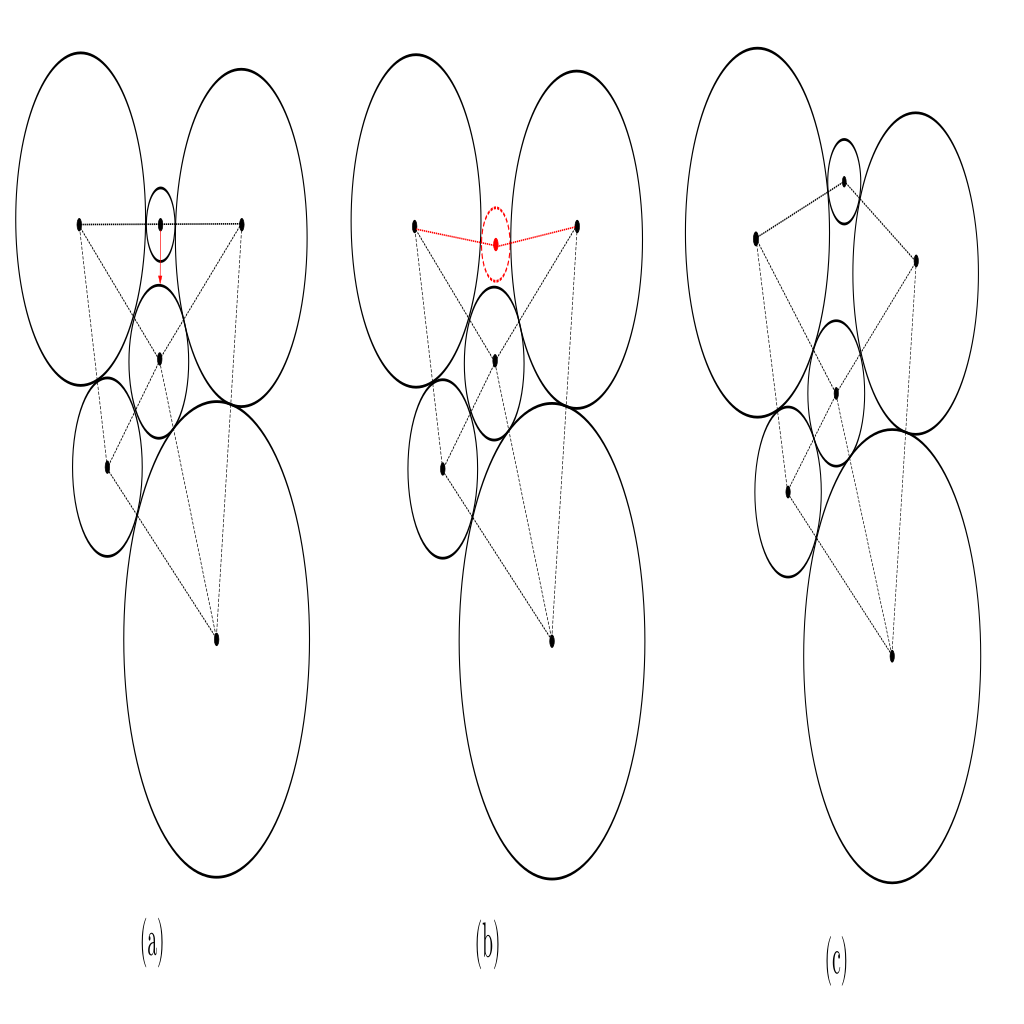
\includegraphics[width = 0.8\textwidth]{Chapter 4/2. Isomorphic but not inf rigid.png}
    \caption{Two isomorphic frameworks. (a) Can be deformed by applying instantaneous velocities (marked in red) on the inner nodes. (b) An infinitesimally rigid framework isomorphic to the one in (a).}
    \label{fig4: iso but not rig}
\end{figure}
\vspace{-3mm}
\begin{flushleft}
We try to unpack this question computationally. By finding known, non-trivial examples for which the conjecture holds, we can be fairly confident that it is true. Thus, the two key players here are going to be modules written in Python called \texttt{Rigidity.py} and \texttt{Circle\_Packing.py}. 
\end{flushleft}

\begin{flushleft}
Titled aptly, the module \texttt{Rigidity} takes in a graph and verifies whether it is infinitesimally rigid, and \texttt{Circle\_Packing} takes a planar graph and attempts to find its circle packing using optimization methods. The graphs we'll be analyzing are all Laman graphs on $n \in [3, \hdots, 10]$ vertices.  
\end{flushleft}

\begin{flushleft}
The generation of minimally rigid graphs on $n = 3,4,5$ vertices can be easily done by hand using the Henneberg Constructions from Theorem \ref{def: henneberg}, henceforth abbreviated to $H_1$ and $H_2$ for Type I and Type II respectively. Starting with a Laman graph on 3 vertices (a triangle):
\begin{itemize}
    \item To obtain the Laman graphs on 4 vertices, we can note that applying $H_1$ yields a graph isomorphic to the one we get when applying $H_2$. so there is only one Laman graph on $4$ vertices. 
    \item To obtain the Laman graphs on 5 vertices, we apply $H_1$ and $H_2$ in four combinations to the triangle;
    \vspace{-2mm}
    \begin{itemize}
        \item Apply $H_1$ twice
        \vspace{-2mm}
        \item First $H_1$, and then $H_2$
        \vspace{-2mm}
        \item First $H_2$, and then $H_1$
        \vspace{-2mm}
        \item Apply $H_2$ twice
    \end{itemize}
    \vspace{-2mm}
    However, we can notice that the graph obtained by applying $H_1$ and then $H_2$ is isomorphic to the graph we obtain when we apply $H_2$ followed by $H_1$. So we conclude that there are only three Laman graphs on 5 vertices.
\end{itemize}

\noindent
This is illustrated in Figures \ref{fig4: n = 4 Laman} and \ref{fig4: n = 5 Laman}.
\end{flushleft}
\vspace{-4mm}
\begin{figure}[htbp]
    \centering
    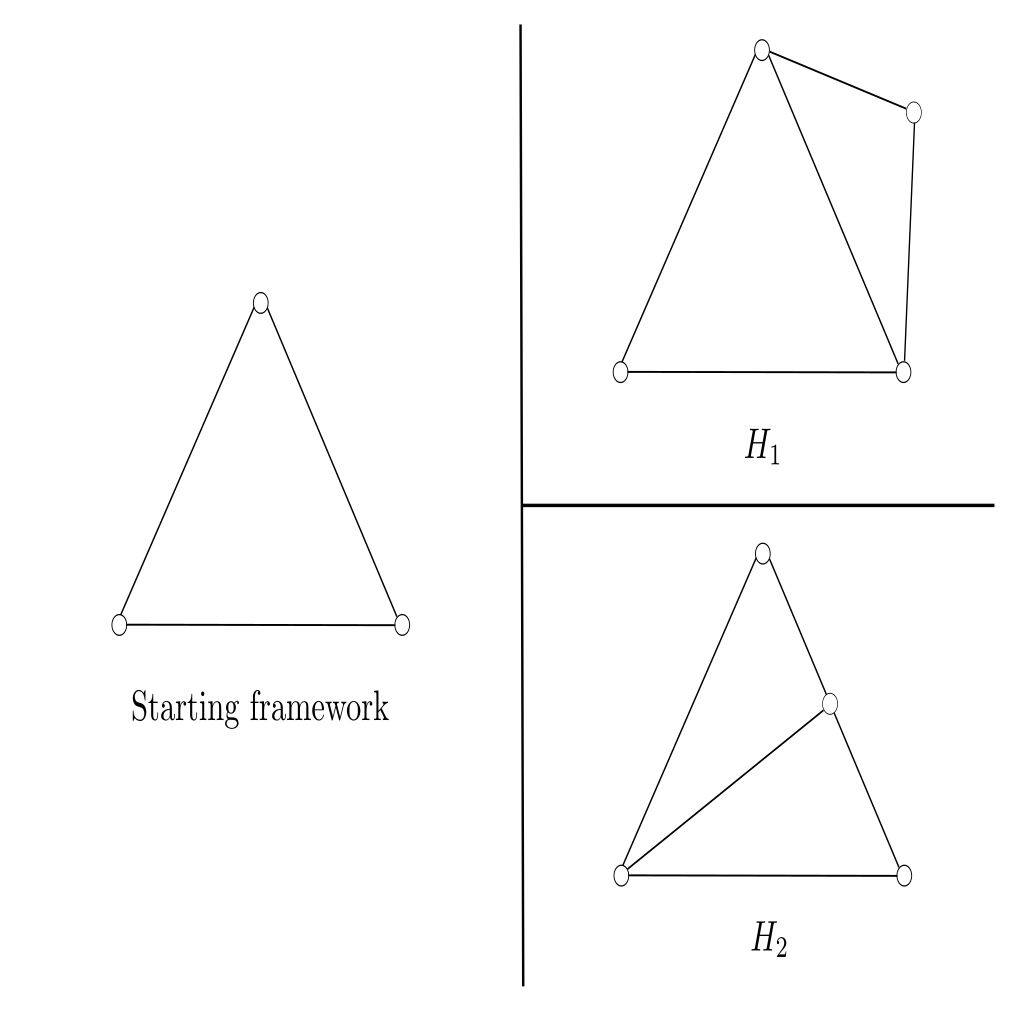
\includegraphics[width = 0.55\textwidth]{Chapter 4/3. n=4.png}
    \caption{Two isomorphic Laman graphs on 4 vertices}
    \label{fig4: n = 4 Laman}
\end{figure}

\begin{figure}[htbp]
    \centering
    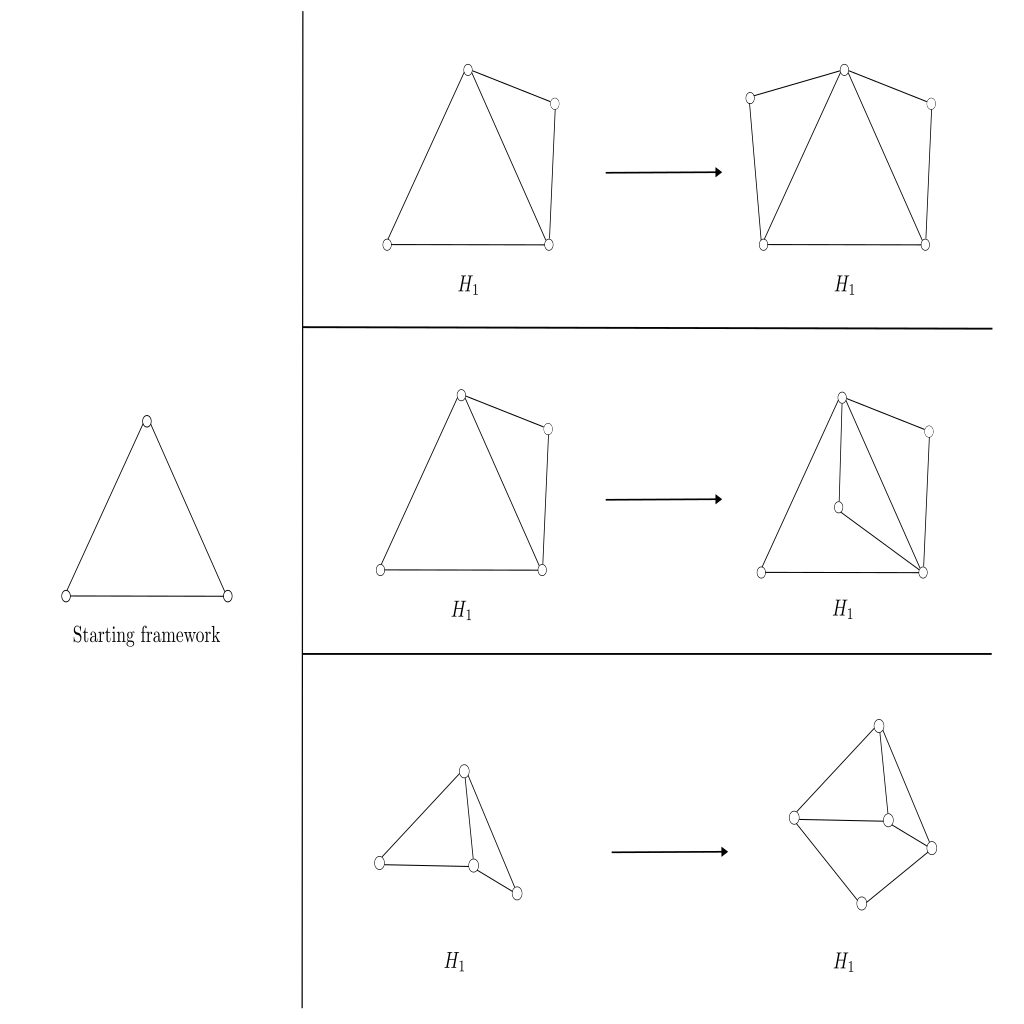
\includegraphics[width = 0.95\textwidth]{Chapter 4/4. n=5.png}
    \caption{Four Laman graphs on 5 vertices. The graphs produced from $H_1 \rightarrow H_2$ and $H_2 \rightarrow H_2$ are isomorphic, so there are three non-isomorphic Laman graphs on 5 vertices.}
    \label{fig4: n = 5 Laman}
\end{figure}


\begin{flushleft}
Planar graphs on vertices $n > 5$ are generated using nauty \cite{nauty}, which allows for the generation of non-isomorphic graphs with a specified number of vertices and edges and saves them as a \texttt{.g6} file. So for example, if we wanted to generate all planar graphs on 8 vertices with 13 edges, we would input
\end{flushleft}

\begin{center}
\texttt{./geng 8 13 | ./planarg | gzip > planar-8-13.g6}    
\end{center}

\noindent
into the terminal. This produces a file named \texttt{planar-8-13.g6}, which contains a list of non-isomorphic planar graphs with the required vertices and edges. At this point, we would invoke the two modules \texttt{Rigidity.py} and \texttt{Circle\_Packing.py} to find the minimally rigid graphs and attempt to pack them. 
\clearpage
\begin{flushleft}
Visually, we can represent what we're trying to do in Figure \ref{fig4: config space}.
\end{flushleft}

\begin{figure}[htbp]
    \centering
    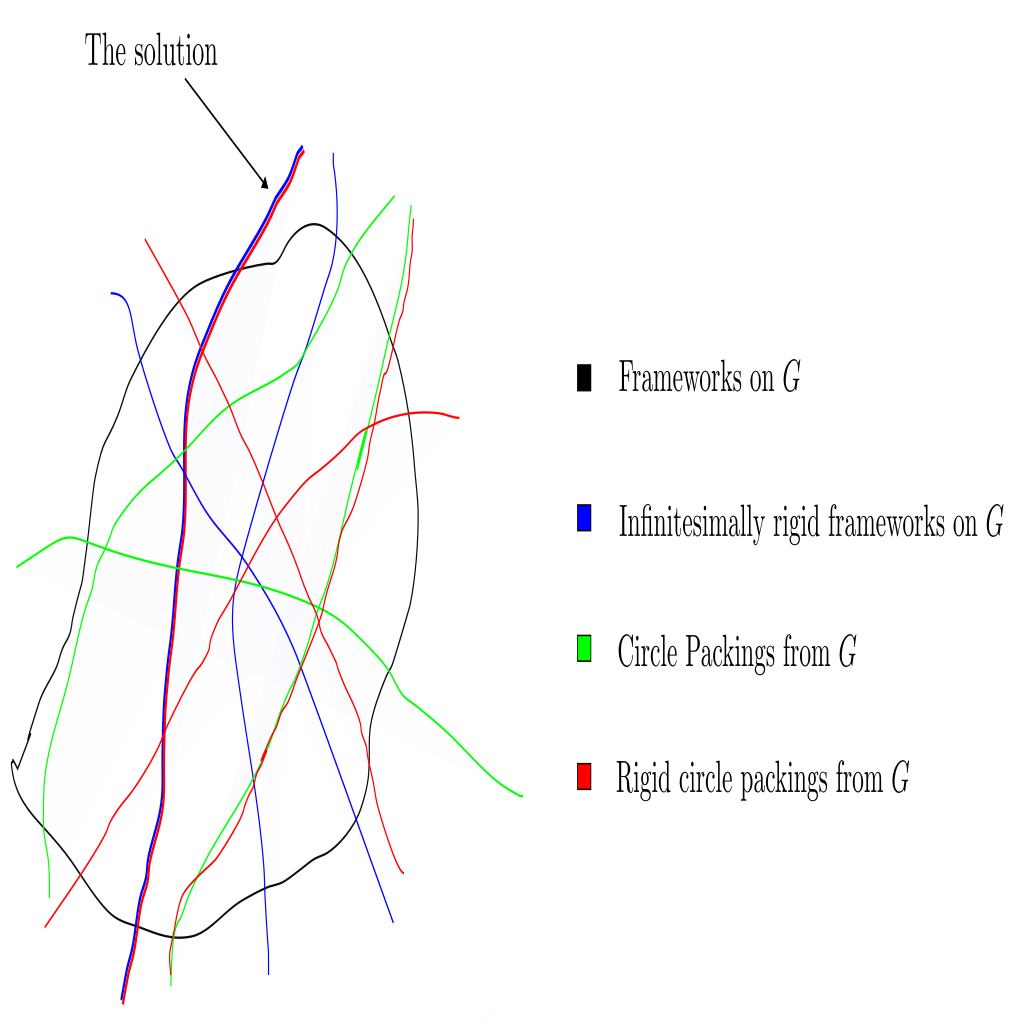
\includegraphics[width = 0.75\textwidth]{Chapter 4/5. configuration space.png}
    \caption{The space containing all frameworks on a graph $G$ drawn as a black outline of the space, the frameworks on $G$ that are infinitesimally rigid drawn as blue lines, the circle packings obtained from $G$ drawn as green lines, and the rigid circle packings obtained from $G$ drawn as red lines.}
    \label{fig4: config space}
\end{figure}

\begin{flushleft}
For a given planar graph $G$ with $n$ vertices and $2n - 3$ edges, there can be a multitude of ways to draw frameworks for it. Referring to Figure \ref{fig4: config space}, we can visualize this as the \textit{space} of frameworks on $G$. Within this space, we have all the frameworks on $G$, some of which are infinitesimally rigid, given as blue lines.  
\end{flushleft}

\begin{flushleft}
Now, for any circle packing obtained from $G$, its underlying contact graph could either be rigid or not, and so we have green lines to represent any circle packing we can get from $G$. Red lines are used to denote what we are after, the rigid circle packings. 
\end{flushleft}

\begin{flushleft}
Thus, the task is to find where the blue and the red lines overlap! That is, we want to find an infinitesimally rigid planar graph such that it produces a circle packing whose contact graph is also infinitesimally rigid (as this implies rigidity). Such an overlap has been made bold in the Figure. 
\end{flushleft}

\begin{flushleft}
Now that we have an understanding of what it is we're trying to do, let us dive into how we go about doing it! By exploring each module individually, we gain an understanding of what is being done. After that, we can go ahead and use the modules in order to find the packings of interest.
\end{flushleft}

\section{\texttt{Rigidity.py}}

\begin{flushleft}
The first module we visit is the one we will be using to check for the rigidity of a given graph. To do this, we will need to compute the rigidity matrix from Theorem \ref{def: rigidity matrix}, and then check whether its rank satisfies Theorem \ref{thm: rank-rigid}. From this point onwards, $n$ shall denote the number of vertices (or nodes) in a graph (or framework), and $m$ shall denote the number of edges in the graph. 
\end{flushleft}

\begin{flushleft}
The graphs we will be considering are made by an existing module in Python known as \texttt{networkx} \cite{networkx}. This module allows for the study and visualization of graphs in Python. Along with this, to create the matrices of interest, we need to use a module called \texttt{numpy} \cite{numpy}. By using built-in structures and functions, such as arrays and functions related to analyzing arrays, we create our rigidity matrix as a \texttt{numpy} array and then use a function to compute its rank.
\end{flushleft}

\begin{flushleft}
This module contains several functions designed to do a particular task, so we visit each of them in turn.
\end{flushleft}

\subsection{Creating a Configuration}

\begin{flushleft}
As touched upon before, a graph is an abstract mathematical object that can be drawn in a multitude of ways. There is no concept of `distance', or the vertices having `coordinates' in $\mathbb{R}^2$. In order to study the rigidity of the graph, we must first take the vertices and give them coordinates, effectively forming a configuration of points. This brings us to the first function in this module, called \texttt{G\_configuration}.
\end{flushleft}

\begin{flushleft}
The function \texttt{G\_configuration} takes in a single argument \texttt{G}, a \texttt{networkx} graph, and begins by learning the number of vertices the graph has. For each vertex then, it randomly assigns an integer for $x$-coordinate and the $y$-coordinate from the interval $[-2^{40}, 2^{40}]$. \textbf{Sampling for coordinates from such a large range of numbers decreases the risk of bias, and increases the variation of points used}\footnote{need a better explanation for why the range is so big}. Finally, it returns two lists, one containing the randomly assigned $x$-coordinates and the other containing the randomly assigned $y$-coordinates.
\end{flushleft}

\begin{flushleft}
Now, we have a number of points, each equipped with their own pair of $(x,y)$ coordinates. The next step is to construct the rigidity matrix.
\end{flushleft}

\subsection{Constructing the Rigidity Matrix}

\begin{flushleft}
We define the function \texttt{rigidity\_matrix} which takes in a graph \texttt{G}, and computes its rigidity matrix with the aid of the function \texttt{G\_configuration}. Recalling Definition \ref{def: rigidity matrix}, the rigidity matrix in $\mathbb{R}^2$ has $m$ rows and $2n$ columns. Knowing this, we can initialise a \texttt{numpy} array on $m$ rows and $2n$ columns, and have every entry in the array be 0.
\end{flushleft}

\begin{flushleft}
The task at this stage is to fill in the appropriate entries of the matrix with the correct values. We use the notation $x_i$ and $y_i$ when talking about the $x$-coordinate and the $y$-coordinate of node $i$ respectively. The computation of the entries of the rigidity matrix is done by using the \texttt{enumerate} function in Python. We keep track of the row index \texttt{i}, as well as the edge \texttt{(u,v)} with each iteration.
\begin{enumerate}
    \item The element in row \texttt{i} and column \texttt{2u} is the $x_u - x_v$.
    \vspace{-3mm}
    \item The element in row \texttt{i} and column \texttt{2u+1} is the $y_u - y_v$.
    \vspace{-3mm}
    \item The element in row \texttt{i} and column \texttt{2v} is the $x_v - x_u$.
    \vspace{-3mm}
    \item The element in row \texttt{i} and column \texttt{2v+1} is the $y_v - y_u$.
\end{enumerate}
The function then returns the rigidity matrix with the modified elements. 
\end{flushleft}

\begin{flushleft}
To test whether this function works as expected, we can try to compute the rigidity matrix of the framework given in Example \ref{eg: rigidity matrix}. This framework has nodes with coordinates $(1,2), (0,0), (2,0)$ and $(1,1)$. 
\end{flushleft}

\begin{flushleft}
By defining the graph \texttt{G} appropriately, and by tweaking the function \texttt{rigidity\_matrix} slightly in order to take the specified coordinates rather than the random ones obtained from \texttt{G\_configuration}, we can compute the rigidity matrix for the example.
\end{flushleft}

\begin{code}
In: print(rigidity_matrix(G))

Out: [[ 1.  2. -1. -2.  0.  0.  0.  0.]    # edge (1,2)
      [ 0.  1.  0.  0.  0.  0.  0. -1.]    # edge (1,4)
      [-1.  2.  0.  0.  1. -2.  0.  0.]    # edge (1,3)
      [ 0.  0. -1. -1.  0.  0.  1.  1.]    # edge (2,4)
      [ 0.  0. -2.  0.  2.  0.  0.  0.]]   # edge (2,3)
\end{code}    

\begin{flushleft}
Comparing this to the rigidity matrix computed by hand in Example \ref{eg: rigidity matrix}, we see that while the order of the edges considered has changed, the entries along each corresponding row have not. Thus, we can safely say the function \texttt{rigidity\_matrix} computes the rigidity matrix for a given graph correctly.
\end{flushleft}

\subsection{Rank of the Rigidity Matrix}

\begin{flushleft}
From Theorem \ref{thm: rank-rigid}, we know that the framework is infinitesimally rigid if and only if the rank of the rigidity matrix is equal to $2n-3$. In order to obtain the rank of a matrix in Python, we make use of the \texttt{linalg} library within \texttt{numpy}. 
\end{flushleft}

\begin{flushleft}
To start, we define a function \texttt{check\_rigidity} which takes a graph \texttt{G}, and calls on the \texttt{rigidity\_matrix} function to get the rigidity matrix of \texttt{G}. From here, we use \texttt{np.linalg.matrix\_rank} to compute the rank of the matrix. If the rank is equal to $2n-3$, the function returns \texttt{True}, and \texttt{False} if the condition fails.
\end{flushleft}

\begin{flushleft}
Considering the framework in Example \ref{eg: rigidity matrix}, we know it is infinitesimally rigid by observation as it is a Laman graph on 4 vertices, and this is infinitesimally rigid by Corollary \ref{cor: laman => inf rigid}. By calling this framework \texttt{G}, let us print the rank of the rigidity matrix of \texttt{G}.
\end{flushleft}

\begin{code}
In: print(np.linalg.matrix_rank(rigidity_matrix(G)))

Out: 5
\end{code}

\begin{flushleft}
As $(2 \times 4) - 3 = 5$, we confirm that this framework is indeed infinitesimally rigid. Now, to verify whether \texttt{check\_rigidity} works as expected, we print its result using \texttt{G} as the argument. 
\end{flushleft}

\begin{code}
In: print(check_rigidity(G))

Out: True
\end{code}

\begin{flushleft}
Thus, we have written a function that now tells us whether a graph is infinitesimally rigid or not.
\end{flushleft}

\subsection{Checking rigidity for a list of graphs}

\begin{flushleft}
Using nauty to generate the graphs we need gives us a list containing all the non-isomorphic planar graphs on a specified number of vertices and edges. Therefore, the last function this module contains is one that filters this list for all the minimally rigid graphs that we want to analyze. In addition to this, we also filter out graphs that have a vertex of degree one or two. 
\end{flushleft}

\begin{flushleft}
If a graph has a vertex with degree one, then it is not rigid and will be discarded when the \texttt{check\_rigidity} function is called. On the other hand, a vertex of degree two can be constructed using a Henneberg Type I construction, we can pack this vertex trivially. Such graphs are not very interesting to look at.
\end{flushleft}

\begin{flushleft}
We start defining the function \texttt{find\_rigid\_graphs} by allowing the argument to be a list of graphs. As the list we are concerned with contains graphs on the same number of vertices, we choose the first graph in the list and let $n$ be the number of vertices in this graph. 
\end{flushleft}

\begin{flushleft}
Now, in order to filter out the graphs containing a vertex of degree of two, we first loop through all the graphs in the list, and then loop through each vertex in each graph. If the graph does \textbf{not} contain a vertex with degree two, then we add it to a separate list called \texttt{graphs\_without\_degree\_2}. 
\end{flushleft}

\begin{flushleft}
From here, we loop through all the graphs in \texttt{graphs\_without\_degree\_2}, check its rigidity using \texttt{check\_rigidity}, and add it to a new list called \texttt{rigid\_graphs}. The function finally returns \texttt{rigid\_graphs}, a list containing all planar minimally rigid graphs of minimum degree atleast three.
\end{flushleft}

\subsection{Testing the code}

\begin{flushleft}
The last thing to do is to ensure that the code works for known examples before we start investigating graphs we know nothing about. Graphs that are not infinitesimally rigid can be seen in Figures \ref{eg: not_rigid} and \ref{eg: not inf rigid 2.0}. For one more graph that is known to be infinitesimally rigid, we consider the Framework in Figure \ref{eg: inf rigid}. We label these graphs \texttt{G1}, \texttt{G2} and \texttt{G3} respectively, and construct them using \texttt{networkx}.
\end{flushleft}

\begin{figure}
    \centering
    \begin{tabular}{c c c}
        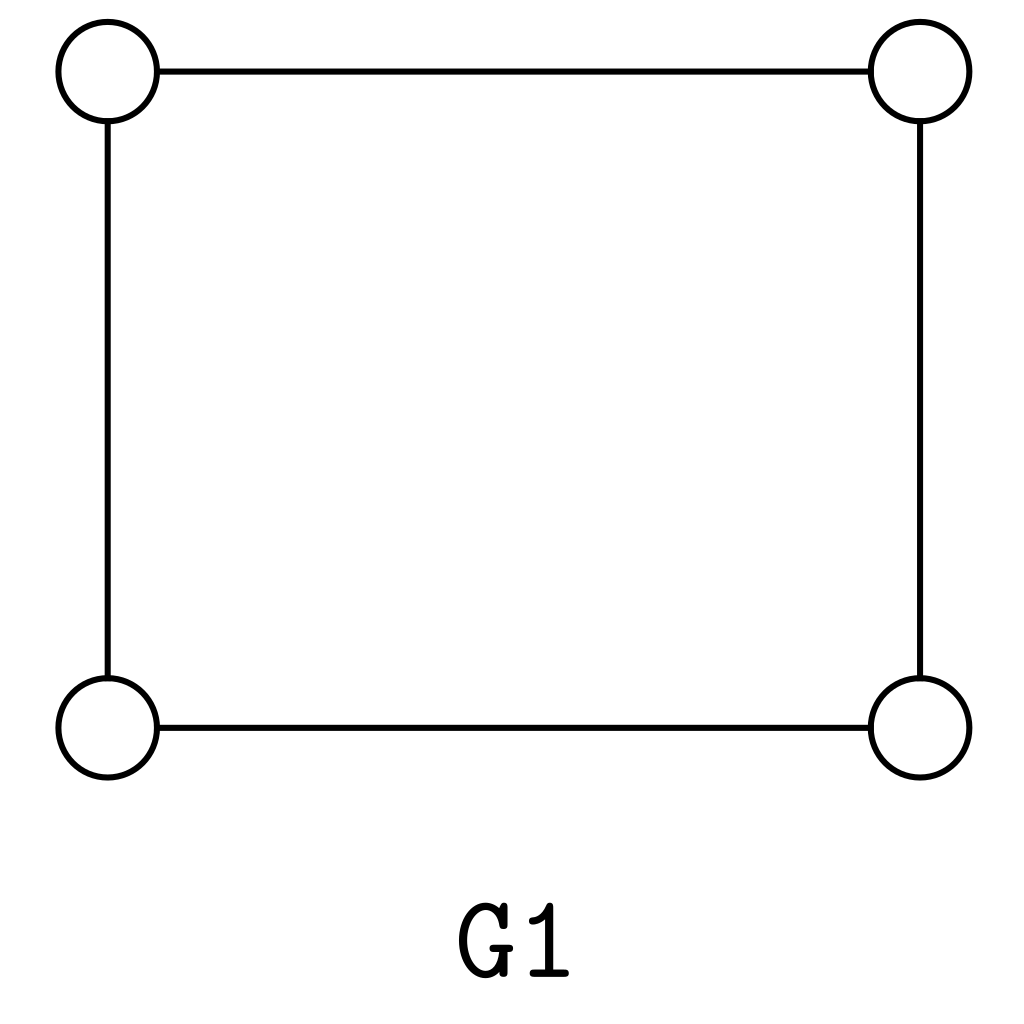
\includegraphics[width = 0.25\textwidth]{Chapter 4/6. not_rigid.png} 
        & 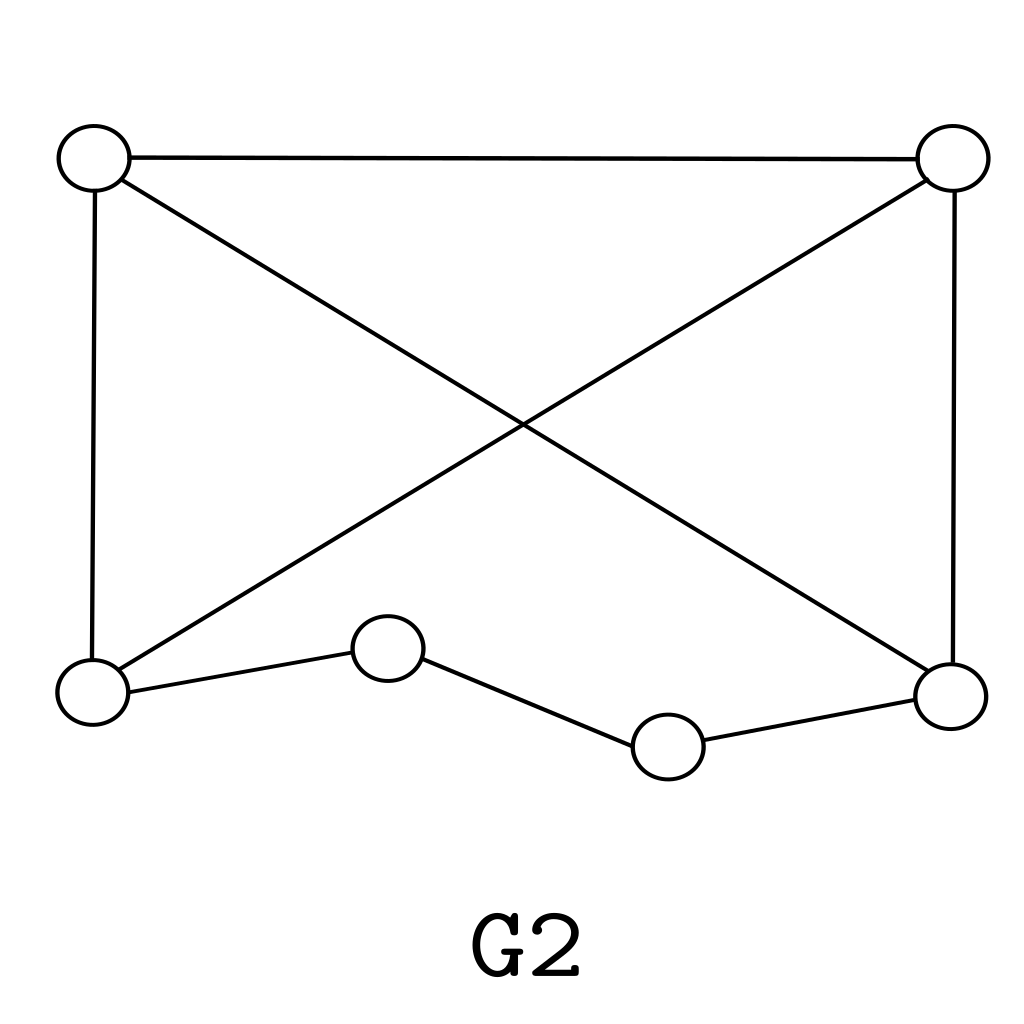
\includegraphics[width = 0.25\textwidth]{Chapter 4/7. not_inf_rigid_2.0.png} &
        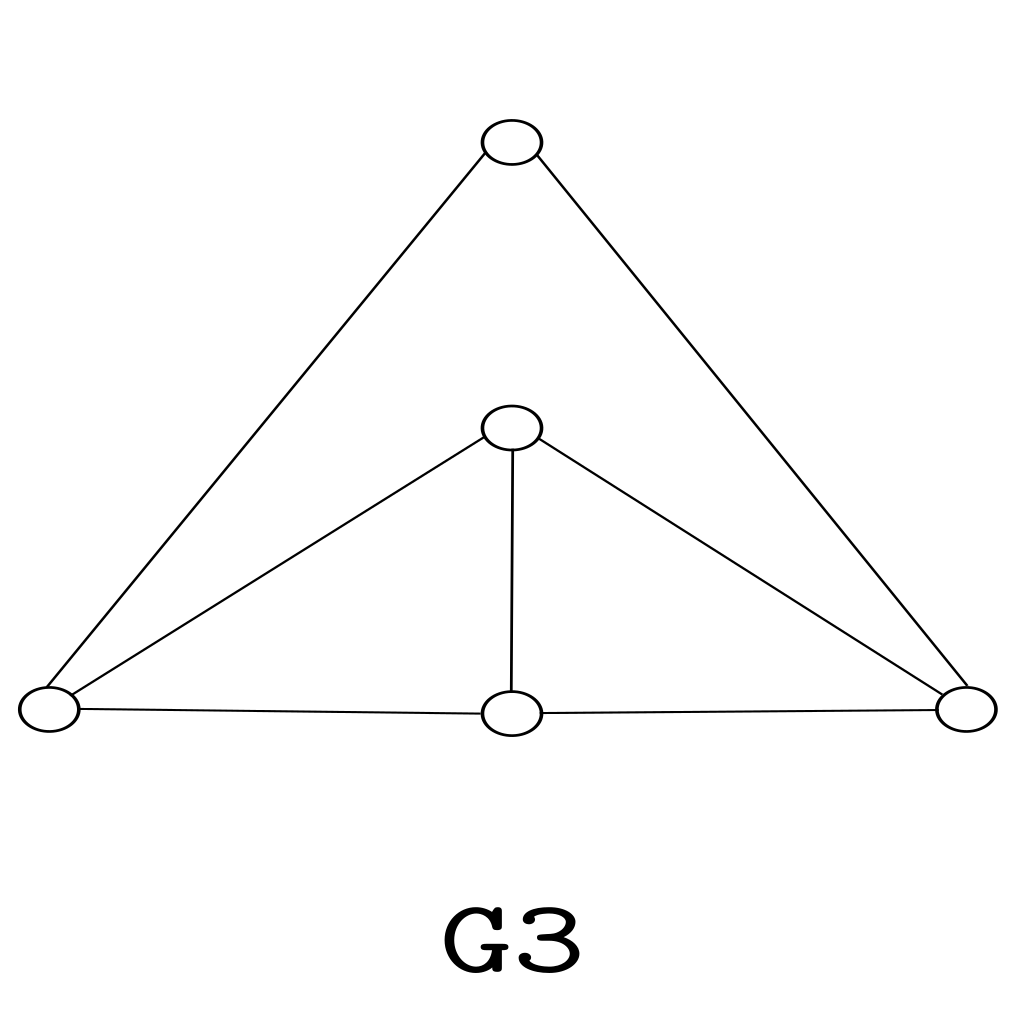
\includegraphics[width=0.2\textwidth]{Chapter 4/8. inf_rigid.png}        
    \end{tabular}
    \caption{The frameworks from Figures \ref{eg: not_rigid}, \ref{eg: not inf rigid 2.0} and \ref{eg: inf rigid} labelled as \texttt{G1}, \texttt{G2}, and \texttt{G3} respectively.}
\end{figure}

\begin{code}
In [1]: print(check_rigidity(G1))
Out: False 

In [2]: print(check_rigidity(G2))
Out: False

In [3]: print(check_rigidity(G3))
Out: True
\end{code}

\begin{flushleft}
This is reassuring to see! We've successfully verified that the functions work well with each other, and that their outputs are as expected. So, with the confidence we have now when it comes to identifying infinitesimally rigid graphs, we can now move onto creating circle packings for a given planar graph. 
\end{flushleft}

\section{\texttt{Circle\_Packing.py}}

\begin{flushleft}
The process of finding circle packings for a graph involves a process called \textit{numerical minimization}. It is a method in which we try to minimize the parameters involved in a given problem with clearly defined rules or \textit{constraints}. In order to find circle packings, we first have to define the problem carefully, and impose certain constraints so that we end up with exactly what we want. Let us briefly run through exactly what this module covers. 
\end{flushleft}

\begin{flushleft}
It is made up of four functions, each performing a specific task, similar to how the functions were defined in \texttt{Rigidity.py}. 
\begin{enumerate}
    \item The first of these functions defines the \textit{objective function} that we want to minimize.
    \vspace{-3mm}
    \item The second function imposes the constraints that the minimization process should obey. 
    \vspace{-3mm}
    \item The third function generates a list of initial conditions that the minimizer will start minimizing.
    \vspace{-3mm}
    \item The very last function is one that uses the three previous functions in order to generate a circle packing for a graph.
\end{enumerate}
\end{flushleft}

\begin{flushleft}
The minimizer that we will be using comes from the \texttt{scipy} \cite{scipy} library in Python called \texttt{scipy.optimize.minimize}. To illustrate how the minimizer works, we describe a simple scenario in which one may use the minimizer in order to minimize a function that is subject to some constraints.
\end{flushleft}

\subsection{A Simple Example}

\begin{flushleft}
\footnote{Should I include this example or not? Maybe consider coding it up}Suppose we have a rectangle of length $x$ and width $y$, and we wish to maximize its area $xy$, subject to the constraint that its perimeter is 20 units. Translating this into something that we can use in the minimizer, the objective function would be $-xy$ as we are trying to maximize the area with the minimize function. The constraint can be modelled as $2x+2y = 20$ and our initial guesses for the values of $x$ and $y$ could be 6 and 4 respectively. We would input this into the \texttt{scipy.optimize.minimize} function, and obtain the optimal values of $x$ and $y$ satisfying these constraints such that the area of the rectangle is minimzed. The code for this example is shown below.
\end{flushleft} 

\begin{code}
# define the objective function
def area_rectangle(xy):
    x = xy[0]
    y = xy[1]
    area = xy[0] * xy[1]
    return -area

# define the constraint
cons = ({'type':'eq', 'fun': lambda xy: 2*xy[0] + 2*xy[1] - 20})

# define the initial condition
initial_guess = [6,4]

# use the minimizer
result = scipy.optimize.minimize(area_rectangle, initial_guess, constraints = cons)

print(f"x = {result.x[0]} and y = {result.x[1]}")
\end{code}

\begin{code}
Out: x = 5.0 and y = 5.0    
\end{code}

\begin{flushleft}
Therefore, the values of $x$ and $y$ that maximize the area of a rectangle with a perimeter of 20 units are 5 and 5 respectively. Hopefully this provides some insight into how the minimizer works. The details of how \texttt{scipy.optimize.minimize} works are not very important for our purposes, but knowing how to use it properly is imperative. 
\end{flushleft}

\begin{flushleft}
With that in mind, let us dive into the first function in the \texttt{Circle\_Packing.py} module!
\end{flushleft}


